
\part*{Vom Konto zur doppelten Buchhaltung}


\section*{Konto}

Herkunft der Namensgebung aus Italienisch: deve dare (soll) und deve
avere (haben).

Darstellung aus der Sicht des Konto-Inhabers:
\begin{verse}
\begin{tabular}{lr|lr}
Soll (Debit) & \multicolumn{2}{c}{} & Haben (Credit)\tabularnewline
\hline 
 &  &  & \tabularnewline
Zugänge &  &  & Abgänge\tabularnewline
 &  &  & \tabularnewline
\end{tabular}
\end{verse}

\section*{Aktiva \& Passiva}

Alles, was einen Beitrag zur Zielerreichung leistet, wird Nutzen genannt.
\begin{quote}
\begin{tabular}{|l|r|}
\hline 
\noun{Aktiv} & \noun{Passiv}\tabularnewline
\hline 
\hline 
Künftigen Nutzenzugang ohne weitere Gegenleistung & Künftiger Nutzenabgang ohne weitere Gegenleistung\tabularnewline
\hline 
\hline 
\emph{Bargeld, Forderungen bei Kunden (Debitoren),} & \emph{Schulden bei Lieferanten (Kreditoren), Banken,}\tabularnewline
\hline 
\hline 
\emph{Vorräte, Maschinen, Fahrzeuge Gebäude etc.} & \emph{Anspr. der Eigentümer}\tabularnewline
\hline 
\end{tabular}
\end{quote}
Ebenfalls ist zu beachten, dass der Saldo bei Aktiv-Konten im Haben
(rechts) verbucht wird, bei Passivkonten im Soll (links)!


\subsection*{Konten für Aktiven}

Aktiv-Konten werden so Dargestellt:
\begin{verse}
\begin{tabular}{lr|lr}
Soll (+) & \multicolumn{2}{c}{\textbf{Aktiv-Konto}} & Haben (-)\tabularnewline
\hline 
 &  &  & \tabularnewline
Anfangsbestand & AB & Abnahme & -\tabularnewline
Zunahme & + & Schlussbestand & SB\tabularnewline
 &  &  & \tabularnewline
 & (Saldo) &  & (Saldo)\tabularnewline
\end{tabular}
\end{verse}

\subsection*{Konten für Passiven}

Passiv-Konten werden so Dargestellt:
\begin{verse}
\begin{tabular}{lr|lr}
Soll (-) & \multicolumn{2}{c}{\textbf{Passiv-Konto}} & Haben (+)\tabularnewline
\hline 
 &  &  & \tabularnewline
Abnahme & - & Anfangsbestand & AB\tabularnewline
Schlussbestand & SB & Zunahme & +\tabularnewline
 &  &  & \tabularnewline
 & (Saldo) &  & (Saldo)\tabularnewline
\end{tabular}
\end{verse}

\subsection*{Bankkonto}

Ein Bankkonto kann sowohl ein Aktiv- (Bankguthaben) oder ein Passiv-Konto
(Bankschuld) sein.

Je nach dem wird im Soll oder im Haben gebucht:
\begin{verse}
\begin{tabular}{|c|c|c|}
\hline 
\noun{Sicht der Unternehmung} & \noun{Buchung der Unternehmung} & \noun{Buchung der Bank}\tabularnewline
\hline 
\hline 
Bankschuld & Buchung im Haben & Buchung im Soll\tabularnewline
\hline 
Bankguthaben & Buchung im Soll & Buchung im Haben\tabularnewline
\hline 
\end{tabular}
\end{verse}
\textbf{ACHTUNG: Besteht eine Bankschuld, so erscheint das Konto in
der Bilanz unter den Passiven!}


\section*{Vom Buchungssatz zur Bilanz}


\subsubsection*{Buchungssatz}

``Buchungstatsachen führen immer zu (mindestens) zwei Konteneinträgen.''


\paragraph*{Soll: }

Zunahme des Vermögens oder Abnahme der Schuld


\paragraph*{Haben:}

Abnahme des Vermögens oder Zunahme der Schuld


\subsubsection*{Buchungstatsache:}
\begin{verse}
\begin{tabular}{|c|c|c|}
\hline 
\noun{Datum} & \noun{Text} & \noun{Betrag}\tabularnewline
\hline 
01.01.2013 & Barbezug vom Postkonto & 50.-\tabularnewline
\hline 
\end{tabular}
\end{verse}

\subsubsection*{Buchungssatz:}
\begin{verse}
\begin{tabular}{|c|c|c|}
\hline 
\noun{Soll-Konto} & \noun{Haben-Konto} & \noun{Betrag}\tabularnewline
\hline 
\hline 
Kasse & Post & 50.-\tabularnewline
\hline 
\end{tabular}
\end{verse}
Journal = Alle Buchungssätze sind in chronologischer Reihenfolge und
komplett.


\subsubsection*{Bilanz}

Die Bilanz ist eine Gegenüberstellung von Aktiven (Vermögen) und Passiven
(Fremd- und Eigenkapital) zu einem bestimmten Zeitpunkt. Man ermittelt
die Salden der Aktiv- und Passivkonten auf einen Bilanzstichtag und
überträgt diese Salden in ein neues Konto, die Bilanz (Diese Buchungen
müssen auch erfasst werden! Buchungen innerhalb der Konten der Bilanz
werden ``Tauschbuchungen'' genannt. Die Unternehmung wird dadurch
nicht ``ärmer'' oder ``reicher''.
\begin{verse}
\begin{tabular}{|c|c|c|}
\hline 
\noun{Beispiel} & \noun{Bezeichung} & \noun{Wirksamkeit}\tabularnewline
\hline 
\hline 
Kasse an Post & Aktivtausch & 0\tabularnewline
\hline 
Lieferantenschuld an Darlehensschuld & Passivtausch & 0\tabularnewline
\hline 
Mobiliar an übr. kurzfr. Schulden & Bilanzverlängerung & +\tabularnewline
\hline 
Bankschuld an Kundenguthaben & Bilanzverkürzung & -\tabularnewline
\hline 
\end{tabular}
\end{verse}

\subsubsection*{Aufbau der Bilanz}
\begin{verse}
\begin{tabular}{lr|lr}
Aktiven & \multicolumn{2}{c}{Bilanz} & Passiven\tabularnewline
\hline 
\multirow{6}{*}{\begin{sideways}
Liquidierbarkeit $\leftarrow$
\end{sideways}} & Umlaufvermögen & kurzfr. Fremdkapital & \multirow{6}{*}{\begin{sideways}
Fristigkeit$\leftarrow$
\end{sideways}}\tabularnewline
 & Anlagevermögen & langfr. Fremdkapital & \tabularnewline
 &  & Eigenkapital & \tabularnewline
 &  &  & \tabularnewline
 &  &  & \tabularnewline
 &  &  & \tabularnewline
\end{tabular}
\end{verse}

\paragraph*{Bilanzverlängerung:}
\begin{quote}
Steigerung der Einnahmen, etc: z.B. Mobiliar auf Kredit gekauft
\end{quote}

\paragraph*{Bilanzverkürzung:}
\begin{quote}
Steigerung des Aufwandes: Bankschulden mit Kundenzahlungen tilgen
\end{quote}

\subsubsection*{Abschlussbuchungen}

Um Aktiv-/Passiv-Konten am Ende des Jahres in die Bilanz zu buchen,
werden folgende Buchungssätze verwendet:
\begin{itemize}
\item Bilanz / Aktivkonto
\item Passivkonto / Bilanz
\end{itemize}

\section*{Konten für Aufwand und Ertrag}

Die Gegenüberstellung der Salden der Aufwand- und Ertragskonten findet
in der Erfolgsrechnung statt. Der Saldo der Erfolgsrechnung wird in
die Bilanz, in die Rubrik ``Eigenkapital'' übertragen. Aufwand-
und Ertragskonten enthalten die Gegenbuchungen zu den in den Aktiven
(Passiven) festgestellten Vermögens-(Schuld-) Zu- und Abnahmen.




\subsection*{Konten für Aufwand}

Aufwand-Konten werden so Dargestellt: Vermögensabnahme oder Schuldzunahme
\begin{verse}
\begin{tabular}{lr|lr}
Soll (+) & \multicolumn{2}{c}{\textbf{Aufwand-Konto}} & Haben (-)\tabularnewline
\hline 
 &  &  & \tabularnewline
 &  & Aufwandminderungen & -\tabularnewline
Zunahme Aufwand & + & Aufwandkorrekturen & -\tabularnewline
 &  &  & \tabularnewline
 &  &  & (Saldo)\tabularnewline
\end{tabular}
\end{verse}

\subsection*{Konten für Ertrag}

Ertrags-Konten werden so Dargestellt: Vermögenszunahme oder Schuldenabnahme
\begin{verse}
\begin{tabular}{lr|lr}
Soll (-) & \multicolumn{2}{c}{\textbf{Ertrags-Konto}} & Haben (+)\tabularnewline
\hline 
 &  &  & \tabularnewline
Ertragsminderungen & - & Zunahme Ertrag & +\tabularnewline
Ertragskorrekturen & - &  & \tabularnewline
 &  &  & \tabularnewline
 & (Saldo) &  & \tabularnewline
\end{tabular}
\end{verse}

\section*{Die Erfolgsrechnung}

Erfolg = Gewinn oder Verlust


\paragraph*{BilanzErfolg --}

Sie zeigt Aktiv- und Passiv-Bestände am Schluss bzw. Anfang der Rechnungsperiode.
Sie ist eine Momentaufnahme, denn sie bezieht sich auf einen Zeitpunkt.


\paragraph*{Erfolgsrechnung}

Sie zeigt in einer Rechnungsperiode, also einem Zeitraum, entstandene
Aufwände und Erträge. Sie gibt einen Einblick in das betriebliche
Geschehen der Unternehmung.
\begin{quote}
\begin{tabular}{ll}
\textbf{\noun{Tauschvorgänge, erfolgsunwirksam}} & \textbf{\noun{Erfolgsvorgänge, erfolgswirksam}}\tabularnewline
\begin{tabular}{cc}
\hline 
a+ & a-\tabularnewline
\hline 
p- & p+\tabularnewline
\hline 
a+ & p+\tabularnewline
\hline 
p- & a-\tabularnewline
\hline 
\end{tabular}a=Aktiven, p=Passiven & %
\begin{tabular}{ccc}
\hline 
Erfolg-- & A+ & a-\tabularnewline
\hline 
Erfolg-- & A+ & p+\tabularnewline
\hline 
Erfolg++ & a+ & E+\tabularnewline
\hline 
Erfolg++ & p- & E+\tabularnewline
\hline 
\end{tabular}A=Aufwand, E=Ertrag\tabularnewline
 & %
\begin{tabular}{cc}
 & \tabularnewline
\hline 
a+ & A-\tabularnewline
\hline 
p- & A-\tabularnewline
\hline 
E- & a-\tabularnewline
\hline 
E- & p+\tabularnewline
\hline 
\end{tabular}Korrekturbuchungen\tabularnewline
\end{tabular}
\end{quote}

\subsubsection*{Abschlussbuchungen}

Um Erfolgs-Konten am Ende des Jahres in die Erfolgsrechnung zu buchen,
werden folgende Buchungssätze verwendet:
\begin{itemize}
\item Erfolgsrechnung / Aufwandkonto
\item Ertragskonto / Erfolgsrechnung
\end{itemize}

\section*{Probebilanz}

Beispiel:
\begin{verse}
\includegraphics[angle=90,scale=0.2]{\string"VomKontoZurDoppeltenBuchhaltung/2013-01-15 11.33.52-2\string".png}
\end{verse}

\section*{Übersicht}

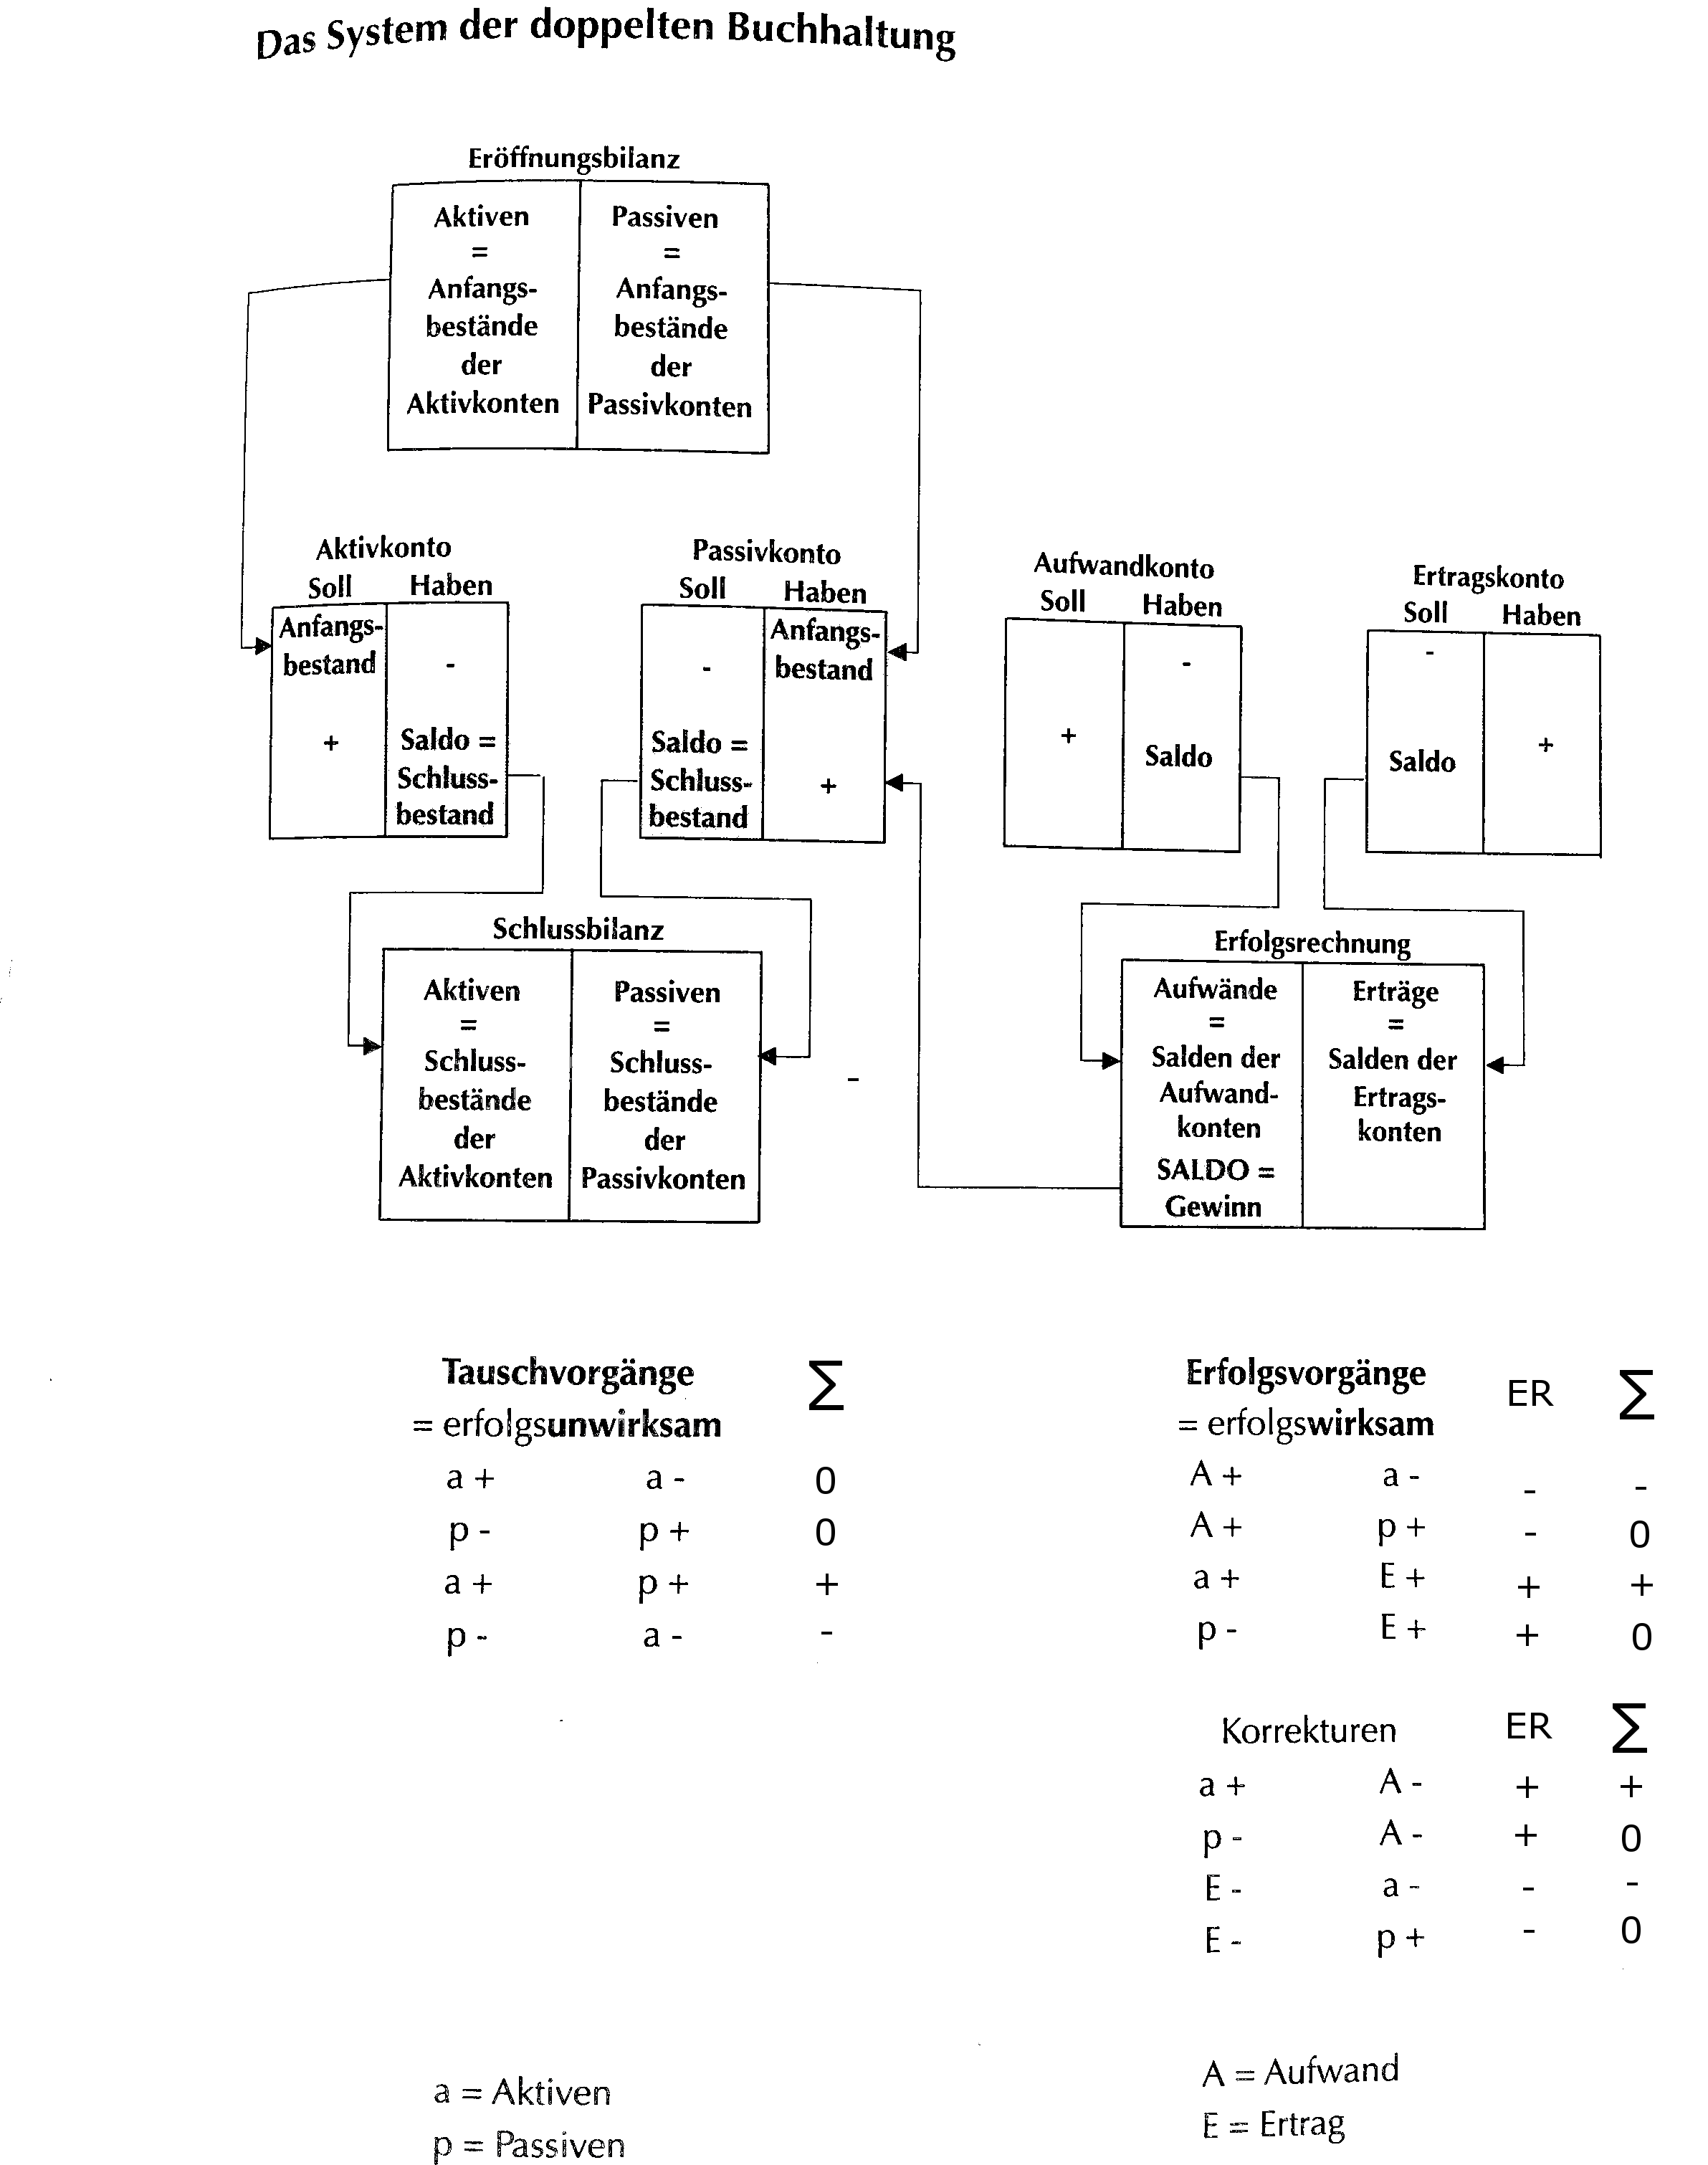
\includegraphics[width=17cm]{VomKontoZurDoppeltenBuchhaltung/DoppelteBuchhaltung}
